\part{Stacks and queues}
\frame{\partpage}

\begin{frame}{Stacks and queues}
	\begin{columns}
		\pause
		\begin{column}{0.3\textwidth}
			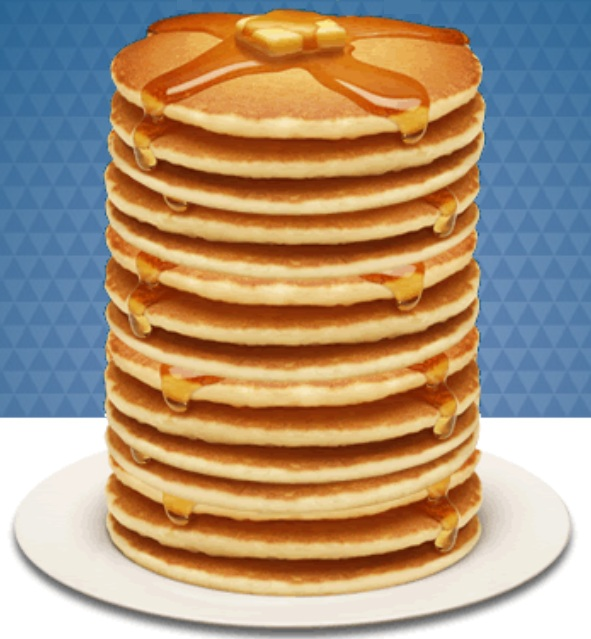
\includegraphics[width=\textwidth]{stack}
		\end{column}
		\begin{column}{0.68\textwidth}
			\begin{itemize}
				\item A \textbf{stack} is a \textbf{last-in first-out (LIFO)} data structure
				\pause\item Items can be \textbf{pushed} to the \textbf{top} of the stack
				\pause\item Items can be \textbf{popped} from the \textbf{top} of the stack
			\end{itemize}
		\end{column}
	\end{columns}
	\begin{columns}
		\pause
		\begin{column}{0.3\textwidth}
			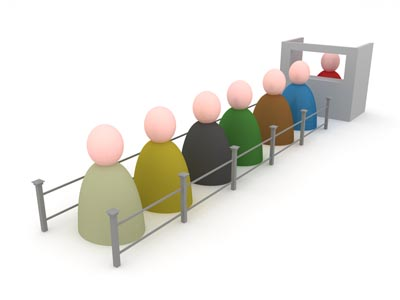
\includegraphics[width=\textwidth]{queue}
		\end{column}
		\begin{column}{0.68\textwidth}
			\begin{itemize}
				\item A \textbf{queue} is a \textbf{first-in first-out (FIFO)} data structure
				\pause\item Items can be \textbf{enqueued} to the \textbf{back} of the queue
				\pause\item Items can be \textbf{dequeued} from the \textbf{front} of the queue
			\end{itemize}
		\end{column}
	\end{columns}
\end{frame}

\begin{frame}[fragile]{Implementing stacks}
	\begin{itemize}
		\pause\item Stacks can be implemented efficiently as lists
		\pause\item Top of stack = end of list
		\pause\item To push an element, use \lstinline{Add} --- $O(1)$ complexity
		\pause\item To pop an element we can do something like this:
			\begin{lstlisting}
x = myStack[myStack.Count - 1];
myStack.RemoveAt(myStack.Count - 1);
			\end{lstlisting}
		\pause\item This is also $O(1)$
	\end{itemize}
\end{frame}

\begin{frame}[fragile]{Implementing queues}
	\begin{itemize}
		\pause\item Queues can be implemented as lists, but not efficiently
		\pause\item End of list = back of queue
		\pause\item Enqueue using \lstinline{Add} --- $O(1)$ complexity
		\pause\item Dequeue by retrieving and removing from beginning of list:
			\begin{lstlisting}
x = myQueue[0];
myQueue.RemoveAt(0);
			\end{lstlisting}
		\pause\item This is $O(n)$
	\end{itemize}
\end{frame}

\begin{frame}[fragile]{Implementing queues}
	\begin{itemize}
		\pause\item End of list = front of queue
		\pause\item Dequeue is like popping from end of list --- $O(1)$ complexity
		\pause\item Enqueue using \lstinline{Insert(0, x)} --- $O(n)$ complexity
	\end{itemize}
\end{frame}

\begin{frame}{Using stacks and queues}
	\begin{itemize}
		\pause\item C\# has \lstinline{Stack} and \lstinline{Queue} classes which you should use instead of trying to use a list
		\pause\item Python has \lstinline{deque} (double-ended queue) which can work as either a stack or a list
	\end{itemize}
\end{frame}

\begin{frame}{Stacks and function calls}
	\begin{itemize}
		\pause\item Stacks are used to implement \textbf{nested function calls}
		\pause\item Each invocation of a function has a \textbf{stack frame}
		\pause\item This specifies information like \textbf{local variable values} and \textbf{return address}
		\pause\item Calling a function \textbf{pushes} a new frame onto the stack
		\pause\item Returning from a function \textbf{pops} the top frame off the stack
		\pause\item Hence the term \textbf{stack trace} when using the debugger or looking at error logs
		\pause\item More on this next week when we look at \textbf{recursion}
	\end{itemize}
\end{frame}
